\documentclass[11pt]{article}
\usepackage{amsfonts}
\usepackage{amsmath}
\usepackage{amssymb}
\usepackage{amsmath}
\usepackage{algorithm}
\usepackage[noend]{algpseudocode}
\usepackage{amsthm}
\usepackage{enumerate}
\usepackage{mathtools}
\usepackage{mathrsfs}
\usepackage{graphicx}
\DeclarePairedDelimiter\abs{\lvert}{\rvert}
\newtheorem{theorem}{Theorem}[section]
\newtheorem{corollary}{Corollary}[theorem]
\newtheorem{lemma}[theorem]{Lemma}
\newtheorem{definition}{Definition}[section]
\makeatletter
\def\BState{\State\hskip-\ALG@thistlm}
\makeatother

\title{\textbf{Primes and How to Recognize them}}
\author{Satwant Rana\\
		2012 MT 50618\\
		Advised by, Prof. Amitabha Tripathi}
\date{}
\begin{document}

\maketitle

\section{Motivation}

Prime numbers are central to Number Theory, acting as the atomic units around which all numbers are built. Therefore it is barely a surprise that \emph{Primality Testing} is a problem with a rich history in Number Theory. 

The motivation behind this project is to rediscover and implement the greatest and the latest in primality testing algorithms.

\section{Primes}

Primes are defined as natural numbers which are only divisible by $1$ and themselves. Formally, given $p \in \mathbb{N}$ is a prime, if whenever $q \mid p$, then $q \in \{1, p\}$.

Any natural greater than $1$ which is not a prime is called a \emph{composite}.

\section{A Naive Primality Test}

The definition of primes presented above can be used to create the simplest primality testing algorithm.\\ Given a natural $n$, whose primality has to determined, we start with $2$ and check for every number upto $n-1$, whether it divides $n$ or not. If we find a divisor in this range, then the above definition tells us that $n$ is not a prime, otherwise it is.

We present the above discussion in pseudocode form in Algorithm~\ref{alg:NaivePrimalityTest}.

\begin{algorithm}
\caption{Naive Primality Test}
\label{alg:NaivePrimalityTest}
\begin{algorithmic}
\Procedure{NaivePrimalityTest}{$n$}
\State $d\gets 2$
\While {$d \leq n-1$}
\State $r \gets n \mod d$
\If {$r = 0$} 
	\State \textbf{return} false \Comment{$n$ is composite}
\EndIf
\State $d \gets d+1$
\EndWhile
\State \textbf{return} true \Comment{$n$ is prime}
\EndProcedure
\end{algorithmic}
\end{algorithm}

The while loop runs over $O(n)$ values, making the runtime of the algorithm linear in $n$. Inside a computer numbers are stored in base $2$ as sequence of bits, and the size of a number is thus determined by its number of bits which is $O(\log n)$. Therefore the above algorithm is exponential in the size of $n$.

\section{An Optimization}
The definition of division in $\mathbb{Z}$ dictates that for $a, n \in \mathbb{Z}$, if $a \mid n$, then there exists $b \in \mathbb{Z}$ such that $n = ab$. Thus, if $a \geq \sqrt n$, then $b \leq \sqrt n$. 

 This reveals that a check for divisors of $n$ upto $\sqrt n$ is sufficient as other divisors would be paired up with one of these divisors. We can optimize the first algorithm we presented to $O(\sqrt n)$ with this optimization, as seen in Algorithm~\ref{alg:OptimizedNaivePrimalityTest}.
 
\begin{algorithm}
\caption{Optimized Naive Primality Test}
\label{alg:OptimizedNaivePrimalityTest}
\begin{algorithmic}
\Procedure{OptimizedNaivePrimalityTest}{$n$}
\State $d\gets 2$
\While {$d \leq \min(n-1,\sqrt n))$}
\State $r\gets n \mod d$
\If {$r = 0$} 
	\State \textbf{return} false \Comment{$n$ is composite}
\EndIf
\State $d \gets d+1$
\EndWhile
\State \textbf{return} true \Comment{$n$ is prime}
\EndProcedure
\end{algorithmic}
\end{algorithm}

\section{Compositeness Tests}
So far we have seen tests which check whether a given number is prime or not. But there exists tests which run much faster than the primality tests discussed above, but on some rare occasions indicate composites as primes. These composite numbers which the compositeness test labels as primes are called the \emph{pseudoprimes} for the test.

More formally, a successful \emph{primality test} proves that a given number is prime, whereas a successful \emph{compositeness test} proves that a given number is composite. 

If a compositeness test is not successful, then we can't comment on the primality of the given number. So how do we use a compositeness test to test primality? We will see in coming sections.

Before we proceed to present some compositeness tests, we need some number theoretic background.

\section{Fermat's (Little) Theorem}

An important and beautiful result in Number Theory, commonly referred to as \emph{Fermat's Little Theorem}, is as presented as Theorem~\ref{theorem:FermatLittleTheorem}.

\begin{theorem}[Fermat's Theorem]
\label{theorem:FermatLittleTheorem}
Given prime $p$, and $a \in \mathbb{Z}$, $(a,p) = 1$ we have,
\[ a^{p-1} \equiv 1 \mod p \]
\end{theorem}

\begin{proof}
If $p \mid a$, then $a^p \equiv a \equiv 0 \mod p$, and we are done. Otherwise if $(a,p) = 1$, then list all the first $p-1$ multiples of $a$,
\[ a, 2a, 3a, \dots (p-1)a\]

All of these numbers are unique $\mod p$, for if $ia \equiv ja \mod p$ then since $(a,p) = 1$, we can cancel $a$ from both sides giving $i \equiv j \mod p$. So, the above numbers represent the following sequence in some order,
\[ 1, 2, 3, \dots (p-1)\]

We can equate the products of the sequences to get, 
\[(p-1)!\ a^{p -1}\equiv (p-1)! \mod p\]

Again since $((p-1)!,p) = 1$, we can cancel $(p-1)!$ to get
\[a^{p-1} \equiv 1 \mod p\]

which completes the proof.
\end{proof}

\begin{corollary}
\label{corollary:BetterFermatLittleTheorem}
Given prime $p$, and $a \in \mathbb{Z}$ we have,
\[ a^p \equiv a \mod p \]
\end{corollary}
 
\begin{proof}
If $(a,p) = 1$, then we have $a^{p-1} \equiv 1 \mod p$ by Theorem~\ref{theorem:FermatLittleTheorem}. We can multiply on both sides by $a$ to get $a^p \equiv a \mod p$.

If $p \mid a$, then $a^p \equiv 0 \equiv a \mod p$. 
\end{proof}

\begin{corollary}
\label{corollary:FermatLittleTheoremConverse}
If $n \in \mathbb{N}$, $n \geq 2$ and $\exists a \in \mathbb{Z}$ such that,
\[a^n \not\equiv a \mod n\]
then $n$ is not a prime.  
\end{corollary}
Corollary~\ref{corollary:FermatLittleTheoremConverse} states the converse of Corollary~\ref{corollary:BetterFermatLittleTheorem}.

\section{Fermat's Theorem as a Compositeness Test}

The Corollary~\ref{corollary:FermatLittleTheoremConverse} is a simple compositeness test using \emph{Fermat's Theorem}. For instance, for $n = 9$, $2^9 \equiv 8 \not\equiv 2 \mod 9$, indicating the compositeness of $9$.

However, there do exist combinations of $a$ and composite $n$ which satisfy the \emph{Fermat's Theorem}. For instance $n = 341 = 11.31$ gives $2^{341} \equiv 2 \mod 341$. This makes $341$ a pseudoprime to the Fermat's Compositeness Test, or a \emph{Fermat Pseudoprime}. Although, in this case a change of base $a$ from $2$ to $3$ yields $3^{341} \equiv 168 \not\equiv 3 \mod 341$ which indicates that $341$ is not a prime.

We arrive at this fallacy because the condition in Corollary~\ref{corollary:FermatLittleTheoremConverse} is only a sufficient condition for $n$ to be a composite, but not a necessary one. And that is what makes it a compositeness test and not a primality test.

As a matter of fact, there do exist composites $n$ which satisfy Corollary~\ref{corollary:FermatLittleTheoremConverse} for all $a$ coprime to $n$, and are called \emph{Carmichael Numbers}. Formally defined, $n$ is a Carmichael Number if $a^{n-1} \equiv 1 \mod n$, $\forall a \in \mathbb{Z}, (a,n) = 1$. The smallest example of Carmichael Numbers is $561$, and there exist infinitely many of them. 

If we add an additional check of whether $(a,n) \neq 1$ in the beginning of the test, we can correctly label Carmichael Numbers as composites given a suitable base $a$ (which is not coprime to $n$).

Let's have some algorithmic buildup before we can present the pseudocode of Fermat's Compositeness Test.

\section{Eucledian Algorithm for G.C.D.}

In this section we present the well-known euclidean algorithm to calculate the greatest common divisor of two (non-negative) integers. Since gcd is defined to be positive, the negative sign can be eliminated by taking absolute values at beginning.

We trivially have $(a,0) = a$, $(a,b) = (a,b-a)$ and therefore $(a,b) = (a,b \mod a)$. 

This set of identities can be leveraged to formulate a systematic way to calculate $(a,b)$, $\forall a, b \in \mathbb{Z}$. If we $b \geq a$, then it can be replaced by $b \mod a$ without affecting the gcd value. Since $b \mod a < a$, we have that the sequence of the minimum of the two numbers is a strictly decreasing one. This assures that the minimum value will finally become $0$, and the algorithm will terminate.

Let's look at the pseudocode in Algorithm~\ref{alg:EuclideanAlgorithm}.

\begin{algorithm}
\caption{Euclidean Algorithm}
\label{alg:EuclideanAlgorithm}
\begin{algorithmic}
\Procedure{EuclideanAlgorithm}{$a, b$}
\State $a \gets \Call{Abs}{a}$
\State $b \gets \Call{Abs}{b}$ \Comment{Eliminating negative signs}
\If {$a > b$}
	\State \Call{Swap}{$a, b$} 
\EndIf
\While {$a \neq 0$}
	\State $c \gets b \mod a$
	\State $b \gets a$
	\State $a \gets c$
\EndWhile
\State \Return $b$
\EndProcedure
\end{algorithmic}
\end{algorithm}

Let's define $a_n, b_n$ to be two numbers at the $i^{th}$ iteration, such that $0 \leq a_n \leq b_n$. We have $a_{n+1} = b_n \mod a_n$, $b_{n+1} = a_n$ and $a_{n+2} = a_n \mod (b_n \mod a_n)$, $b_{n+2} = b_n \mod a_n$. Thus either $a_{n+1} \leq \frac {a_n} 2$, or $a_{n+2} = a_n - a_{n+1} \leq \frac {a_n} 2$. 

Therefore, the minimum of the two numbers gets halved in atmost two steps, making the algorithm take $O(\log \min(\abs a,\abs b))$ remainder calculation steps.

\section{Logarithmic Exponentiation}

An essential part of the Fermat's Compositeness Test is to be able to calculate the value $a^n$. We can calculate it by repeatedly multiplying $a$ to a running product $n$ times and calculating the remainder modulo $n$. This is an $O(n)$ algorithm to calculate $a^n$, thus making Fermat's Composteness Test $\Omega(n)$ in time - not an improvement over primality tests discussed so far.

Fortunately, there's structure to the problem in the form of the following recursion
\[a^n = \begin{cases} 
      1 & n = 0 \\
      (a^{\frac n 2})^2 & n \equiv 0 \mod 2 \\
      a(a^{\frac {n-1} 2})^2 & n \equiv 1 \mod 2 \\
   \end{cases}
\]

The above can be rewritten in the form of Algorithm~\ref{alg:RecursiveLogarithmicExponentiation}.

\begin{algorithm}
\caption{Recursive Logarithmic Exponentiation}
\label{alg:RecursiveLogarithmicExponentiation}
\begin{algorithmic}
\Procedure{RecursiveLogarithmicExponentiation}{$a, n, m$} 
\State $result \gets 1 \mod m$ \Comment{Calculates $a^n \mod m$}
\If {$n > 0$ \ \& \ $n \equiv 0 \mod 2$}
	\State $result \gets \Call{RecursiveLogarithmicExponentiation}{a, \frac n 2, m}$
	\State $result \gets result * result \mod m$ \Comment{Watch for overflow here}
\ElsIf {$n > 0$ \ \& \ $n \equiv 1 \mod 2$}
	\State $result \gets \Call{RecursiveLogarithmicExponentiation}{a, \frac {n-1} 2, m}$
	\State $result \gets result * result \mod m$
	\State $result \gets result * a \mod m$
\EndIf
\State \Return $result$
\EndProcedure
\end{algorithmic}
\end{algorithm}

At every step of recursion, the value of $n$ gets halved thus the algorithm takes $O(\log n)$ multiplication steps.

We can improve on Algorithm~\ref{alg:RecursiveLogarithmicExponentiation}, by eliminating the recursion. Computers store numbers in binary. Suppose $n = b_{d-1}b_{d-2}\dots b_{0} = \sum_{i=0}^{d-1}b_i 2^i$, where $d$ is the number of bits of $n$ and $b_i$ is the $i^{th}$ bit from right. So $a^n$ can be calculated as
\[a^n = a^{\sum_{i=0}^{d-1}b_i 2^i} = \prod_{i=0}^{d-1} a^{b_i 2^i}\]

The above equation can be represented as Algorithm~\ref{alg:IterativeLogarithmicExponentiation}.

\begin{algorithm}
\caption{Iterative Logarithmic Exponentiation}
\label{alg:IterativeLogarithmicExponentiation}
\begin{algorithmic}
\Procedure{IterativeLogarithmicExponentiation}{$a, n, m$}
\State $result \gets 1 \mod m$ \Comment{Calculates $a^n \mod m$}
\State $b \gets a$
\While {$n > 0$}
\If {$n \mod 2 = 1$} \Comment{If rightmost bit is 1 }
	\State $result \gets result * b \mod m$ \Comment{Multiply by $b$}
\EndIf
\State $b \gets b * b \mod m$ \Comment{$b$ stores $a^{2^i}$ on $i^{th}$ step}
\State $n \gets \frac n 2$ \Comment{Remove rightmost bit}
\EndWhile \label{euclidendwhile}
\State \Return result
\EndProcedure
\end{algorithmic}
\end{algorithm}
Thus we can write Fermat's Compositeness Test as Algorithm~\ref{alg:FermatCompositenessTest}.

\begin{algorithm}
\caption{Fermat's Compositeness Test}
\label{alg:FermatCompositenessTest}
\begin{algorithmic}
\Procedure{FermatCompositenessTest}{$a, n$}
\State $gcd \gets \Call{EucledianAlgorithm}{a, n}$.
\If {$gcd > 1 \ \& \ gcd < n$}
	\State \Return $false$
\EndIf
\State $left \gets \Call{IterativeLogarithmicExponentiation}{a,n,n}$
\State $right \gets a \mod m$
\State \Return $left \neq right$
\EndProcedure
\end{algorithmic}
\end{algorithm}

It's easy to see that the algorithm takes $O(\log n)$ time.

\section{Fermat's Theorem as a Probabilistic Primality Test}

Once we have a compositeness test, we can run a it for a fixed number of times on the same number (with changing parameters). If we don't get indication of compositeness even a single time, then the probability of the given number being a composite is too low, and we have a \emph{Probabilistic Primality Test}. A probabilistic primality test thus indicates whether a number is composite or a \emph{probable prime}, i.e. a number which is prime with some (high) probability.

This technique can be applied to Fermat's Compositeness Test, by changing the base $a$ on successive iterations, as seen in Algorithm~\ref{alg:FermatProbabilisticPrimalityTest}.

\begin{algorithm}
\caption{Fermat's Probabilistic Primality Test}
\label{alg:FermatProbabilisticPrimalityTest}
\begin{algorithmic}
\Procedure{FermatProbabilisticPrimalityTest}{$n, iter$} 
\While {$iter > 0$} \Comment {$iter$ is number of iterations}
	\State $a \gets \Call{Random}{0,n-1}$ \Comment {Random number in the range $[0,n-1]$}
	\State $check \gets \Call{FermatCompositenessTest}{a,n}$
	\If {check}
		\State \Return $false$ \Comment {Composite found}
	\EndIf
	\State $iter \gets iter-1$
\EndWhile
\State \Return $true$ \Comment {Probable prime found}
\EndProcedure
\end{algorithmic}
\end{algorithm}

A small value of $iter = 20$ works well in practice, and thus we have an $O(\log n)$ algorithm.

\section{Fermat's theorem as a Primality Test}
When trying to convert a compositeness test into a primality test, the first obvious solution that comes to mind is to (somehow) maintain a table of all possible pseudoprimes within the range we wish to work on. Before running the actual test, one can lookup the table to see if the input number is a pseudoprime for the test, and label it as a composite right at the beginning of the test.

The pseudoprimes for Fermat's Test also depend upon the base $a$ other than input $n$. D.H. Lehmer prepared a table of all Fermat pseudoprimes below $2.10^8$ for the base $2$ with no factor $< 317$. Thus a primality test to check primality for $n < 2.10^8$ can be formulated as Algorithm~\ref{alg:FermatPrimalityTest}.

\begin{algorithm}
\caption{Fermat's Primality Test}
\label{alg:FermatPrimalityTest}
\begin{algorithmic}
\Procedure{FermatPrimalityTest}{$n$} 
\If {$n \geq 2.10^8$}
	\State \Return $false$ \Comment {Fail if out of range}
\EndIf
\For {$i = 2$, $i \leq \min(313,n-1)$, $i \gets i+1$}
	\If {$i \mid n$}
		\State \Return $false$ \Comment {Factor $\leq 313$}
	\EndIf
\EndFor
\If {$\Call{IterativeLogarithmicExponentiation}{2,p-1,p} \not\equiv 1 \mod 2$}
	\State \Return $false$ \Comment {Composite by Fermat's Theorem}
\EndIf
\State \Return $!\Call{IsLehmerPseudoprime}{n}$ \Comment {Check Lehmer's Table}
\EndProcedure
\end{algorithmic}
\end{algorithm}

\section{A Generalisation of Fermat's Little Theorem}
Fermat's Little Theorem is only a necessary condition for a number to be prime, and therefore we can only formulate compositeness tests with it.

What if there were a necessary and sufficient version of it? Then we could use the sufficiency condition to formulate a primality test.

We present one such generalisation of Fermat's Little Theorem.

\begin{theorem}
\label{theorem:GeneralisedFermatLittleTheorem}
Given $n \in \mathbb{N}$, $n \geq 2$ and $a \in \mathbb{Z}$, $(a,n) = 1$, then $n$ is prime if and only if
\[ (X+a)^n \equiv X^n + a \mod n \]
\end{theorem}

\begin{proof}
For $0 < i < n$, the coefficient of $X^i$ in the polynomial $(X+a)^n - (X^n + a)$ is ${n \choose i} a^{n-i}$, and for $i = 0$, it's $a^n - a$.

If $n$ is a prime, then ${n \choose i} \equiv 0 \equiv a^n - a \mod n$, so the polynomial is identically $0 \mod n$.

If $n$ is a composite with a prime factor p such that $p^q || n$, then $p^q \not | {n \choose p}$ and is comprime to $a^{n-q}$.
% ellaborate the part above
And so the coefficient of $X^p$ is not $0 \mod n$, making the above polynomial not identically $0 \mod n$.
\end{proof}
This gives us a simple primality test for input $n$. We chose an appropriate $a$, and evaluate the terms of the polynomial $(X+a)^n -(X^n + a) \mod n$. We have $O(n)$ terms and so the primality test is atleast $\Omega(n)$. Can we do better? Specifically, can we find a polynomial time algorithm?

\section {Building up to a Polynomial Time Primality Test}
It's clear that we need to reduce the number of terms in the aforementioned polynomial. One simple way to reduce terms is to consider the polynomial modulo $X^r - 1$ for some small $r$. That is we make use of the identity,
\[(X+a)^n \equiv X^n + a \mod (n, X^r - 1)\] 
The above equation stands for $(X+a)^n - (X^n + a) = nP(X) + (X^r - 1)Q(X)$ for some polynomials $P$ and $Q$.

From Theorem~\ref{theorem:GeneralisedFermatLittleTheorem} we know that the above equation is satisfied by all primes $n$. But we can have composite $n$ and some choice of $a$ and $r$, for which the above equation true. 

Agarwal, Kayal and Saxena proved that if for several choices of $a$ and for some fixed $r$ the above equation is satisfied, then $n$ is power of a prime. We present their work in the following sections about the \emph{AKS Primality Test}. Further the value of $r$ and number of choices for $a$ are both polynomial in $\log n$.

\section {The AKS Primality Test}
Without much further ado, we present to you the \emph{AKS Primality test} as Algorithm~\ref{alg:AKSPrimalityTest}.

\begin{algorithm}
\caption{AKS Primality Test}
\label{alg:AKSPrimalityTest}
\begin{algorithmic}
\Procedure{AKSPrimalityTest}{$n$} 

\If {$n < 2$ or $n = a^b$ for $a, b \in \mathbb{N}$ and $b \geq 2$}
	\State \Return $false$  \Comment {Step 1}
\EndIf

\State $r \gets min \{i: i \in \mathbb{N},\ i \leq \max(3,\ \lceil \log^5 n \rceil),\ o_i(n) > \log^2 n \}$ \Comment {Step 2}

\For {$a = 2$, $a \leq r$, $a \gets a+1$}
	\If {$1 < (a,n) < n$}
		\State \Return $false$  \Comment {Step 3}
	\EndIf
\EndFor

\If {$n \leq r$}
	\Return $true$  \Comment {Step 4}
\EndIf

\For {$a = 1$, $a \leq \lfloor \sqrt{\phi(r)} \log n \rfloor$, $a \gets a+1$}
	\If {$(X+a)^n \not \equiv X^n + a \mod (n, X^r - 1)$}
		\State \Return $false$  \Comment {Step 5}
	\EndIf
\EndFor
\State \Return $true$ \Comment {Step 6}
\EndProcedure
\end{algorithmic}
\end{algorithm}


In the coming sections we string a series of lemmas to formulate the proof for AKS.

\begin{lemma}
\label{lemma:AKSLemma1}
If $n$ is a prime then Algorithm~\ref{alg:AKSPrimalityTest} returns $true$.
\end{lemma}
 
\begin{proof}
If $n$ is a prime, then Steps $1$ and $3$ can never return $false$. Also by discussion in previous section, Step $5$ can't return $false$. So the algorithm returns $true$ in either Step $4$ or Step $6$.
\end{proof}

\subsection{Is $n$ a perfect power?}
The check for Step $1$ can be done in $O(\log^3 n)$ arithmetical operations. We need to find whether there exist $a, b \in \mathbb{N}, b \geq 2$ such that $n = a^b$. The idea is as follows. We iterate over all $1 \leq b \leq \log n$ and binary search for the root $a$ of the equation $n = a^b$. 

We present the details in Algorithm~\ref{alg:PerfectPowerTest}. It involves $\log n$ iterations for $b$, $\log n$ iterations for binary search, and $\log n$ arithmetic operations for logarithmic exponentiation. So, overall it takes $O(\log^3 n)$ arithmetic operations to check if $n$ is a perfect power. Numbers can take as much as $\log n$ space, so it takes $\tilde O(\log n)$ time for arithmetic operations, and $\tilde O(\log^4 n)$ time overall. Here $\tilde O(f(n)) = O(f(n) \cdot \log^{\epsilon} f(n))$, for some constant $\epsilon$.

\begin{algorithm}
\caption{Perfect Power Test}
\label{alg:PerfectPowerTest}
\begin{algorithmic}
\Procedure{PerfectPowerTest}{$n$}
\If {$n = 1$}
	\State \Return $true$
\EndIf
\For {$b \gets 2$, $b \leq \log n, b \gets b+1$}
	\State $l \gets 1, u \gets n$
	\While {$l < u$}
		\State $m \gets \lfloor \frac{l+u}{2} \rfloor$
		\State $x \gets m^b$ \Comment{Use Logarithmic Exponentiation here}
		\If {$x = n$}
			\ \Return $true$
		\ElsIf {$x < n$}
			\ $l \gets m+1$
		\Else
			\ $r \gets m-1$
		\EndIf
	\EndWhile
\EndFor
\State \Return $false$
\EndProcedure
\end{algorithmic}
\end{algorithm}


\subsection {Existence of a small $r$}
In this section, we prove that there exists an $r$ as required in Step $2$.

\begin{lemma}
\label{lemma:LCMLemma}
Let $LCM(m)$ be $lcm$ of first $m$ numbers. We have for $m \geq 7$,
\[LCM(m) \geq 2^m\]
\end{lemma}
%%\begin{proof}
%%To Be Added
%%\end{proof}

\begin{lemma}
\label{lemma:AKSLemma2}
There exists an $r \leq \max(3, \lceil \log^5 n \rceil)$ and $o_r(n) > \log^2 n$.
\end{lemma}
\begin{proof}
If $n = 2$, then $r = 3$ works. Assume $n \geq 3$. Let $B = \lceil \log^5 n \rceil$. Since $n \geq 3$, we have $B > 10$. 

Consider the smallest $r \in \mathbb{N}$ which doesn't divide the product $P$ defined as,
\[P = n^{\log B}\ .\ \prod_{i=1}^{\lfloor \log^2 n \rfloor}{n^i-1} \]

We have,
\[n^{\log B}\ .\ \prod_{i=1}^{\lfloor \log^2 n \rfloor}{n^i-1} < n^{\log B + \sum_{i=1}^{\log^2 n}i} \leq n^{\log^4 n} \leq 2^{\log^5 n} \leq LCM(B)\]
Second inequality holds for $n \geq 2$ and last inequality follows by Lemma~\ref{lemma:LCMLemma}. If $r > B$, then it can't be the smallest natural not dividing $P$ as $P < LCM(B)$. Hence, $r \leq B$.

Now, let $p$ be a prime factor of $r$, such that $p^q || r$. So that $q \leq \log r \leq \log B$. If $p | n$, then $p^q | n^{\log B}$. Since $r \not | P$, there exists one prime $p | r$ such that $p \not | n$. As $p \ |  \frac{r}{(n,r)}$ and therefore, $\frac{r}{(n,r)} \not | P$. Since $r$ is the smallest natural not dividing $P$, so $r \leq \frac{r}{(n,r)}$. Therefore $(n,r) = 1$. 

Now we can define $o_r(n)$. Since $n^i \not \equiv 1 \mod r \ \forall \ r \leq \lfloor \log^2 n \rfloor$, we have $o_r(n) > \log^2 n$.
\end{proof}

\subsection{Some definitions}
We have shown that Algorithm~\ref{alg:AKSPrimalityTest} returns $true$ if input $n$ is a prime. What remains to be shown is that it returns $false$ if $n$ is composite.

Since $n > 2$, $o_r(n) > 1$. So there exists a prime divisor $p$ of $n$ such that $o_r(p) > 1$. Since $(n,r) = 1$, we have $(p,r) = 1$. Also, $p > r$ else Step $3$ or $4$ would identify that. For the rest of the discussion we would keep $p$ and $r$ fixed. Also let $l = \lfloor \sqrt{\phi(r)} \log n \rfloor$.

Now what remains to be shown is that if any of the equations in Step $5$ is $true$, then $n$ is not a prime. If $n$ satisfies all the $l$ conditions of Step $5$ then,
\[(X+a)^n \equiv X^n + a \mod (n, X^r - 1)\ \forall\ 0 \leq a \leq l \ \ \ \ \dagger\]

Or in other words $(X+a)^n = X^n + a$ in the ring $\mathbb{Z}_n[X]/(X^r-1)$ for all $0 \leq a \leq l$. Note that $X$ acts as a primitive $r^{th}$ root of unity in $\mathbb{Z}_n[X]/(X^r-1)$.

From Theorem~\ref{theorem:GeneralisedFermatLittleTheorem},
\[(X+a)^p \equiv X^p + a \mod (n,X^r-1)\]
From $\dagger$ we have, 
\[((X+a)^p)^{\frac{n}{p}} \equiv (X^p)^{\frac{n}{p}} + a \mod (n, X^r - 1)\ \forall\ 0 \leq a \leq l \]
By combining the last two equations we get,
\[(X^p+a)^{\frac{n}{p}} \equiv (X^p)^{\frac{n}{p}} + a \mod (n, X^r - 1)\ \forall\ 0 \leq a \leq l \]

Since $X$ is a primitive $r^{th}$ root of unity in $\mathbb{Z}_n[X]/(X^r-1)$ and $(p,r) = 1$, $X^p$ is also a primitive $r^{th}$ root of unity in $\mathbb{Z}_n[X]/(X^r-1)$. So, $X = X^{pq}$, where $pq \equiv 1 \mod r$. Therefore,
\[(X^p+a)^{\frac{n}{p}} \equiv (X^p)^{\frac{n}{p}} + a \mod (n, (X^p)^r - 1)\ \forall\ 0 \leq a \leq l \] Conversely, every primitive $r^{th}$ root of unity can be arrived at in this fashion. And therefore,
\[(X+a)^{\frac{n}{p}} \equiv X^{\frac{n}{p}} + a \mod (n, X^r - 1)\ \forall\ 0 \leq a \leq 
l \]

So we conclude that both $p$ and $\frac{n}{p}$ satisfy $\dagger$. The \emph{AKS} algorithm gives a name to this property,

\begin{definition}
\label{definition:introspective}
For polynomial $f(X)$ and $m \in \mathbb{N}$, if $m$ satisfies
\[f(X)^m \equiv f(X^m) \mod (n,X^r-1)\]
then $m$ is said to be introspective for $f(X)$.
\end{definition}

\begin{lemma}
\label{lemma:IntrospectiveLemma1}
If $m$ and $m'$ are both introspective for a polynomial $f(X)$, then so is $m . m'$.
\end{lemma}
\begin{proof}
Since $m$ is introspective for $f(X)$, we have
\[f(X)^m \equiv f(X^m) \mod (n, X^r-1)\]
Substituting $X^{m'}$ for $X$ in the above equation, we have
\[f(X^{m'})^m \equiv f((X^{m'})^m) \mod (n, (X^{m'})^r-1)\]
Also since $m'$ is introspective for $f(X)$, we have
\[f(X)^{m'} \equiv f(X^{m'}) \mod (n, X^r-1)\]
Combining the two equations, we get
\[f(X)^{mm'} \equiv f(X^{mm'}) \mod (n, X^{m'r}-1)\]
Since $X^{r}-1 | X^{m'r}-1$,
\[f(X)^{mm'} \equiv f(X^{mm'}) \mod (n, X^r-1)\]
\end{proof}
\begin{lemma}
\label{lemma:IntrospectiveLemma2}
If $m$ is introspective for both the polynomials $f(X)$ and $g(X)$, then it is also introspective for $f(X) . g(X)$.
\end{lemma}
\begin{proof}
We have,
\[f(X)^m \equiv f(X^m) \mod (n, X^r-1)\]
\[g(X)^m \equiv g(X^m) \mod (n, X^r-1)\]
Multiplying together,
\[f(X)^mg(X)^m \equiv f(X^m)g(X^m) \mod (n, X^r-1)\]
which is nothing but,
\[(f(X)g(X))^m \equiv f(X^m)g(X^m) \mod (n, X^r-1)\]
\end{proof}

\subsection{About two groups}
The previous two lemmas put together imply that the every number in the set $I = \{\frac{n}{p}^i.p^j\ |\ i,j \in \mathbb{N}_0\}$ for every polynomial in the set $P = \{\prod_{a=0}^{l}{(X+a)^{e_a}}\ |\ e_a \in \mathbb{N}_0\}$. These two sets help define two groups which play a vital role in the analysis of \emph{AKS}.

The first group is the set of residues of all elements of $I$ modulo $r$. Let's denote this set as $G$, and it is a subset of $\mathbb{Z}_r^*$ as $(n,r) = (p,r) = 1$. Let $t = |G|$. Since $n^i \in G \ \forall \ i \in \mathbb{N}_0$ and $o_r(n) > \log^2(n)$, we have $t > \log^2(n)$.

Now over to the definition of the second group. Let $Q_r(X)$ be $r^{th}$ cyclotomic polynomial over $F_p$. $Q_r(X)$ divides $X^r-1$ and factors into irreducible factors of degree $o_r(p)$ in $F_p$. Let $h(X)$ be one such irreducible factor. Since $o_r(p) > 1$, degree of $h(X)$ is greater than one. The second group is the set of all residues of polynomials in $P$ modulo $h(X)$ and $p$. Let $\mathcal{G}$ be this group. This group is generated by elements $X, X + 1, X + 2, \dots, X + l$ in the field $F = F_p[X]/(h(X))$ and is a subgroup of the multiplicative group of $F$.
%%Proof for degree of h, and F is a field
\subsection{Estimating the size of $\mathcal{G}$}
\begin{lemma}
[Lenstra]\label{lemma:GLowerBound}
$|\mathcal{G}| \geq {{t+l} \choose {t-1}}$
\end{lemma}
\begin{proof}
We begin by reminding that since $h(X)$ is a factor of $Q_r(X)$, $X$ is a primitive $r^{th}$ root of unity.

We show that any two distinct polynomials $f(X), g(X) \in P$ with degree less than $t$, map to different elements in $\mathcal{G}$. Let's assume to the contrary that $f(X) = g(X)$ in $F$. Let $m \in I$. We also have $f(X)^m = g(X)^m$ in $F$. Since $m$ is introspective for $f(X)$ and $g(X)$, and $h(X)$ divides $X^r-1$, we have $f(X^m) = g(X^m)$ in $F$. So, $X^m$ is a root of the the polynomial $Q(Y) = f(Y) - g(Y)$ in $F$, for every $m \in G$ (as $h(X)$ divides $X^r-1$). Now $G \subset \mathbb{Z}_r^*$, so $(m,r) = 1$, and hence $X^m$ is a distinct primitive $r^{th}$ root of unity for every $m \in G$. This means that $Q(Y)$ has atleast $t = |G|$ roots in $F$. However the degree of $Q(Y)$ is less than $t$ because of the choice of $f(X)$ and $g(X)$. Hence, $f(X) \neq g(X)$ in $F$.

Now, if $0 \leq i \neq j \leq l$ then $i \neq j$ in $F_p$ as $l = \lfloor \sqrt{\phi(r)} \log n\rfloor < \phi(r) < r < p$. The first inequality is true becuase $\log^2{n} < o_r(n) < \phi(r)$. So $X, X+1, X+2, \dots, X+l$ are all distinct in $F = F_p[X]/(h(X))$. Also since degree of $h(X)$ is greater than $1$, $X+a \neq 0\ \forall \ 0 \leq a \leq l$. Therefore, there are atleast $l+1$ distinct polynomials of degree $1$ in $\mathcal{G}$.

We can now estimate the number of polynomials of degree less than $t$ in $F$. The set $P_t = \{\prod_{a=0}^{l}(X+a)^{e_a}\ | \ \sum_{a=0}^{l}e_a \leq t-1\}$ is a subset of the set of polynomials with degree $<t$ in $\mathcal{G}$, and $|P_t| = {{l+t}\choose{t-1}}$. As discussed above all these polynomials are distinct in $\mathcal{G}$, and therefore $|\mathcal{G}| \geq {{t+l} \choose {t-1}}$.
\end{proof}

\begin{lemma}
\label{lemma:GUpperBound}
If $n$ is not a power of $p$, then $|\mathcal{G}| \leq n^{\sqrt{t}}$
\end{lemma}
\begin{proof}
Consider the subset of $I$, $I' = \{p^i.(\frac{n}{p})^j\ |\ 0 \leq i, j \leq \lfloor \sqrt{t} \rfloor \}$.
Since $n$ is not a power of $p$, $I'$ has $(\lfloor \sqrt{t} \rfloor + 1)^2 > t$ numbers. Since $|G| = t$, two of the members of $I'$ must be equal modulo $r$. Let $m_1, m_2$ with $m_1 > m_2$ be the numbers. 

So we have, $X^{m_1} \equiv X^{m_2} \mod (n, X^r-1)$. Using this and the fact that $m_1, m_2$ are intospective for any $f(X) \in P$, we have 
\[f(X)^{m_1} \equiv f(X^{m_1}) \equiv f(X^{m_2}) \equiv f(X)^{m_2} \mod (n, X^r-1)\]
Therefore, $f(X)^{m_1} = f(X)^{m_2}$ in $F$ for all $f(X) \in P$. 

Consider the polynomial $Q'(Y) = Y^{m_1} - Y^{m_2}$ over the field $F$. Since every member of $\mathcal{G}$ is a root of $Q'(Y)$, we have that $Q'(Y)$ has atleast $|\mathcal{G}|$ roots in $F$. The degree of $Q'(Y)$ is $m_1$, so $|\mathcal{G}| \leq m_1$.

By the definition of $I'$, $m_1 \leq (p.\frac{n}{p})^{\sqrt{t}} = n^{\sqrt{t}}$. Therefore, $|\mathcal{G}| \leq n^{\sqrt{t}}$.

\end{proof}

\subsection{Completing the proof}
\begin{lemma}
\label{lemma:CombinationsLemma}
\[{2n+1 \choose n} \geq 2^{n+1}\]
\end{lemma}
\begin{proof}
\[{2n+1 \choose n} = \frac{\prod_{i=1}^{n}(n+1+i)}{\prod_{i=1}^{n}{i}} = \prod_{i=1}^{n}\frac{n+1+i}{i}\]
\[ = \prod_{i=2}^{n}\frac{n+1+i}{i}\ .\ (n+2) \geq \prod_{i=2}^{n}2\ .\ (n+2) = 2^{n-1}(n+2)\]

Since $n \geq 2$,
\[{2n+1 \choose n} \geq 2^{n-1}(n+2) \geq 2^{n-1}.(4) = 2^{n+1}\]
\[\]
\end{proof}

\begin{theorem}
If Algorithm~\ref{alg:AKSPrimalityTest} returns $true$ then input $n$ is prime.
\end{theorem}
\begin{proof}
Here, we handle the case of $true$ being returned at Step $6$. We make use the last two lemmas,
\[|\mathcal{G}| \geq {{t+l} \choose {t-1}}\]

Since $t > \log^2 n$, and therefore $t > \sqrt t \log n$. Combining with the fact that ${{t+l} \choose {t-1}} = \frac{\prod_{i=0}^l{(t+i)}}{(l+1)!}$ is an increasing function in $t$,
\[|\mathcal{G}| \geq {{{\lfloor \sqrt t \log n \rfloor} + 1 + l} \choose {\lfloor \sqrt t \log n \rfloor}}\]

Also $l = \lfloor \sqrt{\phi(r)} \log n \rfloor$, and $G \subset \mathbb{Z}_r^{*}$. So $t = |G| \leq |\mathbb{Z}_r^{*}| = \phi(r)$. Therefore, $l \geq \lfloor \sqrt{t} \log{n} \rfloor$, and hence,
\[|\mathcal{G}| \geq {{2{\lfloor \sqrt t \log n \rfloor}+1} \choose {\lfloor \sqrt t \log n \rfloor}}\]

Using Lemma~\ref{lemma:CombinationsLemma},
\[|\mathcal{G}| \geq 2^{{\lfloor \sqrt t \log n \rfloor}+1} > 2^{\sqrt t \log n} = n^{\sqrt t}\]

But we know that $|\mathcal{G}| \leq n^{\sqrt t}$ unless $n$ is power of a prime. So $n = p^{q}$ for some power $q$. But if that were the case we would have identified it in Step $1$ of the algorithm. Hence, $n$ is a prime.
\end{proof}

\subsection{Time Complexity analysis}
As discussed before, Step $1$ can be done in $\tilde O(\log^4 n)$ time.

Step $2$ involves calculating if order is greater than $\log^2 n$ for $\log^5 n$ numbers. This can be checked by calculating $n^i$ succesively for $1 \leq i \leq \lceil \log^5 n \rceil$. The size of the numbers can get as large as $\log \log^5 n$. So it takes $\tilde O({\log^5 n} \cdot {\log^2 n}) = \tilde O(\log^7 n)$ time for this step.

Step $3$ is gcd calcuation for numbers as large as $n$, so it can be done in $O(\log^2 n)$ time.

What remains of interest is Step $5$. There are $l = \lfloor \sqrt{\phi(r)} \log n \rfloor = O(r^{1/2} \log n)$ iterations. Each iterations involve exponentiation of polynomials. Each exponentiation takes $O(\log n)$ iterations. There are $O(r)$ terms in each polynomial, and coefficients are as large as $n$. So it takes $\tilde O({r^{3/2} \log^3 n})= \tilde O(\log^{10.5}n)$. This step dominates the time complexity, and hence the time complexity of overall algorithm is $\tilde O(\log^{10.5}n)$

\subsection{Implementation and Simulations}
\begin{figure}
  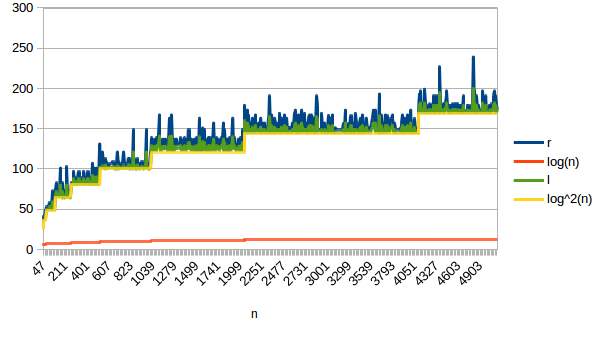
\includegraphics[width=\linewidth]{pictures/n-r-l-5000.png}
  \caption{AKS simulations for $n \leq 5000$.}
  \label{fig:aks_5000}
\end{figure}
An implementation of AKS, in accordance to this text, can be found at \\\texttt{https://github.com/satwantrana/primality-testing}. The code works for input of arbitrary size. The present implementation uses a combination of Quadratic, Karatsuba and Toom-Cook multiplication algorithms for polynomial and integer multiplication and thus the algorithm is slightly slower than the previously discussed complexity.

Figure~\ref{fig:aks_5000} represents the values of $r$ and $l$ against $n$ along the $x$-axis, for $n \leq 5000$. It can be seen that $r \sim \log^2 n$, and therefore $l \sim r$ in this range. These values are much smaller than the upper bound of $\log^5 n$ and much closer to the lower bound of $\log^2 n$. Also, both $r$ and $l$ increase roughly in a step-fuction fashion along with $\log^2 n$. 

Figure~\ref{fig:aks_2000} represents the time taken by the code to evaluate the primality of input $n$, for $n \leq 2000$. The expected number of iterations in the algorithm is $O(\log^{4 + 2\log3} n)$, as $r \sim log^2 n$ and multiplication algorithm for polynomials is Karatsuba in this range. The observed runtimes suggest that the constant of complexity is $\sim 100$. Arbitrary precision arithmetic requires frequent memory references, which explains the large constant. A clever implementation can bring this number down by a factor, but still this shows that AKS is impractical as a primality test even for small numbers. 

The most expensive part of the algorithm is Step $5$, where $l$ equations in $\mathbb{Z}_n[X]/(X^r-1)$ have to be checked. All the numbers which fail this step are composite numbers with no prime factor $\leq r$. A simulation reveals that such $n \leq 1.4 \cdot 10^6$, fail the test at $a = 1$ itself. A further investigation in this direction can lead to smaller value for $l$, which can reduce the overall time complexity of the AKS primality test.

\begin{figure}
  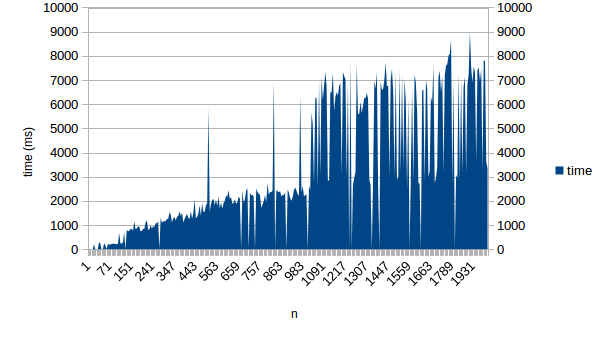
\includegraphics[width=\linewidth]{pictures/n-time-2000.png}
  \caption{AKS simulations for $n \leq 2000$.}
  \label{fig:aks_2000}
\end{figure}

\subsection{A modification of AKS}
If we drop Step 1 from Algorithm~\ref{alg:AKSPrimalityTest}, then the false positives for the primality test can only be composite prime powers, and it becomes a probabilistic primality test. The following lemma describes a probabilistic version of AKS primality test whose false positives can only be composites with atmost $k$ distinct prime divisors.

\begin{lemma}
\label{lemma:AKSGenerelisation1}
Given $k$ and $n$, the following modifications to AKS primality test, result in a probabilistic primality test whose false positives can only be composites with atmost $k$ distinct prime divisors.
\begin{enumerate}[1.]%for capital roman numbers.
\item Choice of $r$ is such that $o_r(n) > \log^{1 + \frac 1 {k}} n$.
\item Such an $r$ would exist with $r \leq \log^{3 + \frac 2 {k}} n$.
\item $l$ is improved to $\lfloor \phi^\frac{1}{k+1}(r) \log n \rfloor$.
\end{enumerate}
Further, the modified algorithm runs in $\tilde O(\log^{3 + (3 + \frac{2}{k})(1 + \frac{1}{k+1})} n)$ time.
\end{lemma}

\begin{proof}
Note that for $k=1$, these bounds are same as the ones mentioned in the AKS primality test. 

In the general setting $r$ is defined to be the smallest natural which doesn't divide the product $P_k$ defined as,
\[P_k = n^{\log B_k}\ .\ \prod_{i=1}^{\lfloor \log^{1 + \frac{1}{k}} n \rfloor}{n^i-1} \]
where $B_k = \lceil \log^{3 + \frac{2}{k}} n \rceil$.

If primes $p_i | n\ \forall \ 1 \leq i \leq k$, then it follows inductively on increasing $j$ that,
\[(X+a)^{n/\prod_{i=1}^{i=j} p_i} \equiv X^{n/\prod_{i=1}^{i=j} p_i} + a \mod (n, X^r - 1)\]
with $1 \leq j \leq k$, using the same arguments as section $14.3$. 

Now, if we modify $I'$ in Lemma~\ref{lemma:GUpperBound} to,
\[I'_k = \{ \prod_{j=1}^{k}p_j^{i_j} \cdot (n/\prod_{j=1}^{k}p_j)^{i_{k+1}} \ \vert \ 0 \leq i_j \leq \lfloor n^\frac{1}{k+1} \rfloor \}\]
and redo the same analysis as the original algorithm, with the corresponding modifications, the result follows.
\end{proof}

As it is, this modified version of AKS isn't very useful, for it's only nominally faster than original AKS. But we see that the choice of $r$ from original AKS satisfies the first two criteria here. Additionally, we know that, from the proof of Lemma~\ref{lemma:AKSGenerelisation1}, after $l_k = \lfloor \phi^\frac{1}{k+1}(r) \log n \rfloor$ iterations in Step $5$ of Algorithm~\ref{alg:AKSPrimalityTest}, the set of false positives is reduced only to composite $n$ with atmost $k$ distinct prime divisors.

\begin{corollary} After $l_k = \lfloor \phi^\frac{1}{k+1}(r) \log n \rfloor$ iterations (from the beginning) in Step 5 of AKS Algorithm, the set of false positives is reduced to composite $n$ with atmost $k$ distinct prime divisors.
\end{corollary}

If we choose to stop at this point, it results in an $\tilde O(\log^{8 + \frac{5}{k+1}} n)$ time probabilistic primality test.

\begin{thebibliography}{9}
\bibitem{riesel} 
Riesel, Hans. 
\textit{Prime Numbers and Computer Methods for Factroization}. Birkhauser, Boston, 1985.
 
\bibitem{aks} 
Agrawal, Manindra; Kayal, Neeraj; Saxena, Nitin. \textit{PRIMES is in P}. Annals of Mathematics, 2004.

 
\bibitem{wikipedia} 
Wikipedia: Primality tests.
\\\texttt{https://en.wikipedia.org/wiki/Primality\_test}
\end{thebibliography}
\end{document}


